\section{Hårdvara}
\subsection{Översikt}
	\begin{center}
		\begin{figure}[H]
    	\centering
			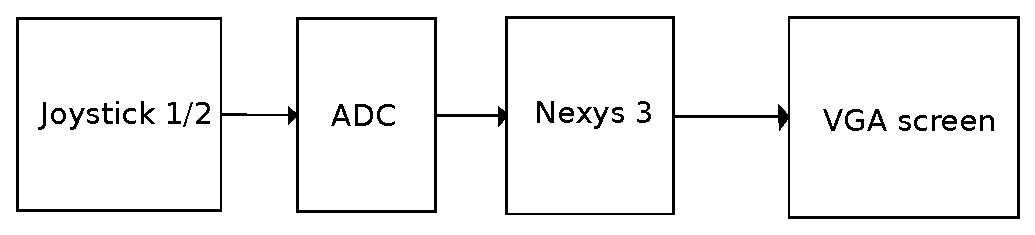
\includegraphics[scale=0.70]{../grafik/overview.eps}
			\caption{Översiktlig design}
			\label{fig:over}
		\end{figure}
	\end{center}
Joystickarna är insignaler till en A/D-omvandlare. Denna omvandlare är sedan i sin tur insignal till Nexys kortet där allt roligt händer. Kortet har en grafikmotor vars utsignal är insignal för en VGA bildskärm. 
\subsection{CPU}
	\begin{center}
		\begin{figure}[H]
    	\centering
			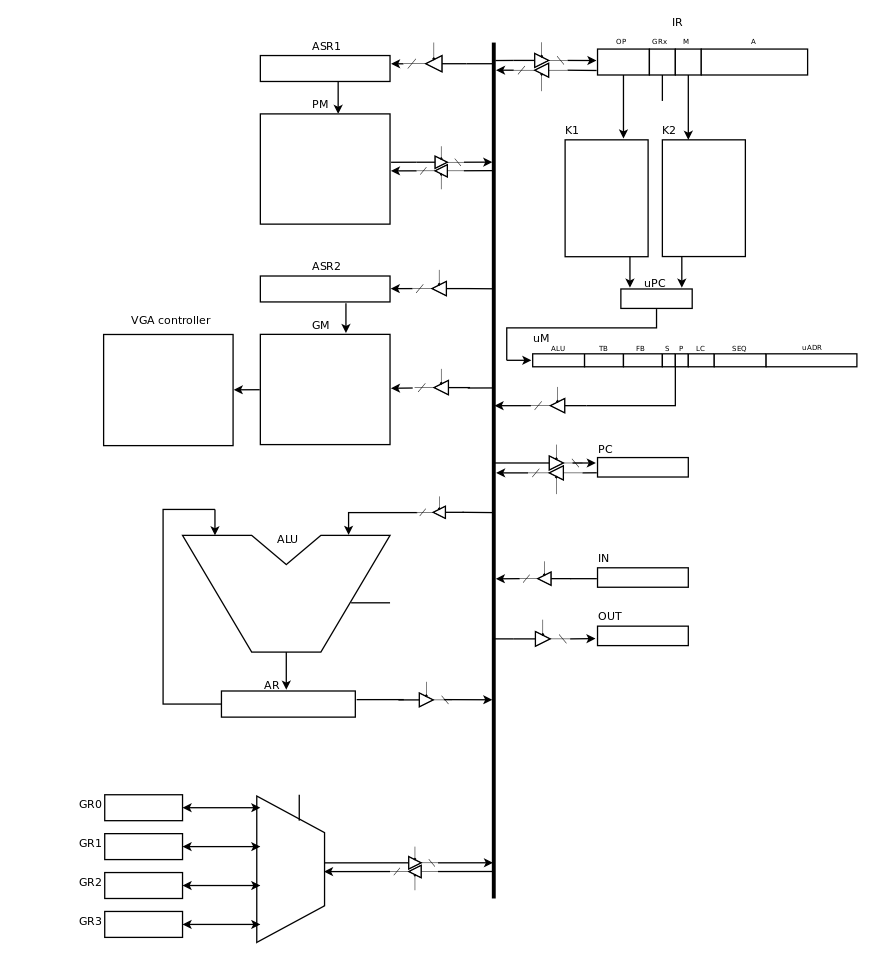
\includegraphics[scale=0.40]{../grafik/overall_design.png}
			\caption{CPU design}
			\label{fig:cpu}
		\end{figure}
	\end{center}
Ovan ses ett översiktligt blockschema på CPU:n. Denna är av Olle Roos modellen och är nästan identisk med CPU:n som användes i laboration 1. Det som lagts till är en grafikdel och en I/O enhet. Instruktionerna som används följer Olle Roos design, med ett par undantag: Instruktionen STOREV har lagts till för att kunna skriva till grafikminnet. Instruktionerna IN och OUT har lagts till för att hantera I/O enheten.
Både program och grafikminne implementerades som Block-RAM i Nexys-kortet. Dessa minnen är lika stora och består av 256 ord à 16 bitar.
\subsection{Grafik}
	\begin{center}
		\begin{figure}[H]
	    \centering
			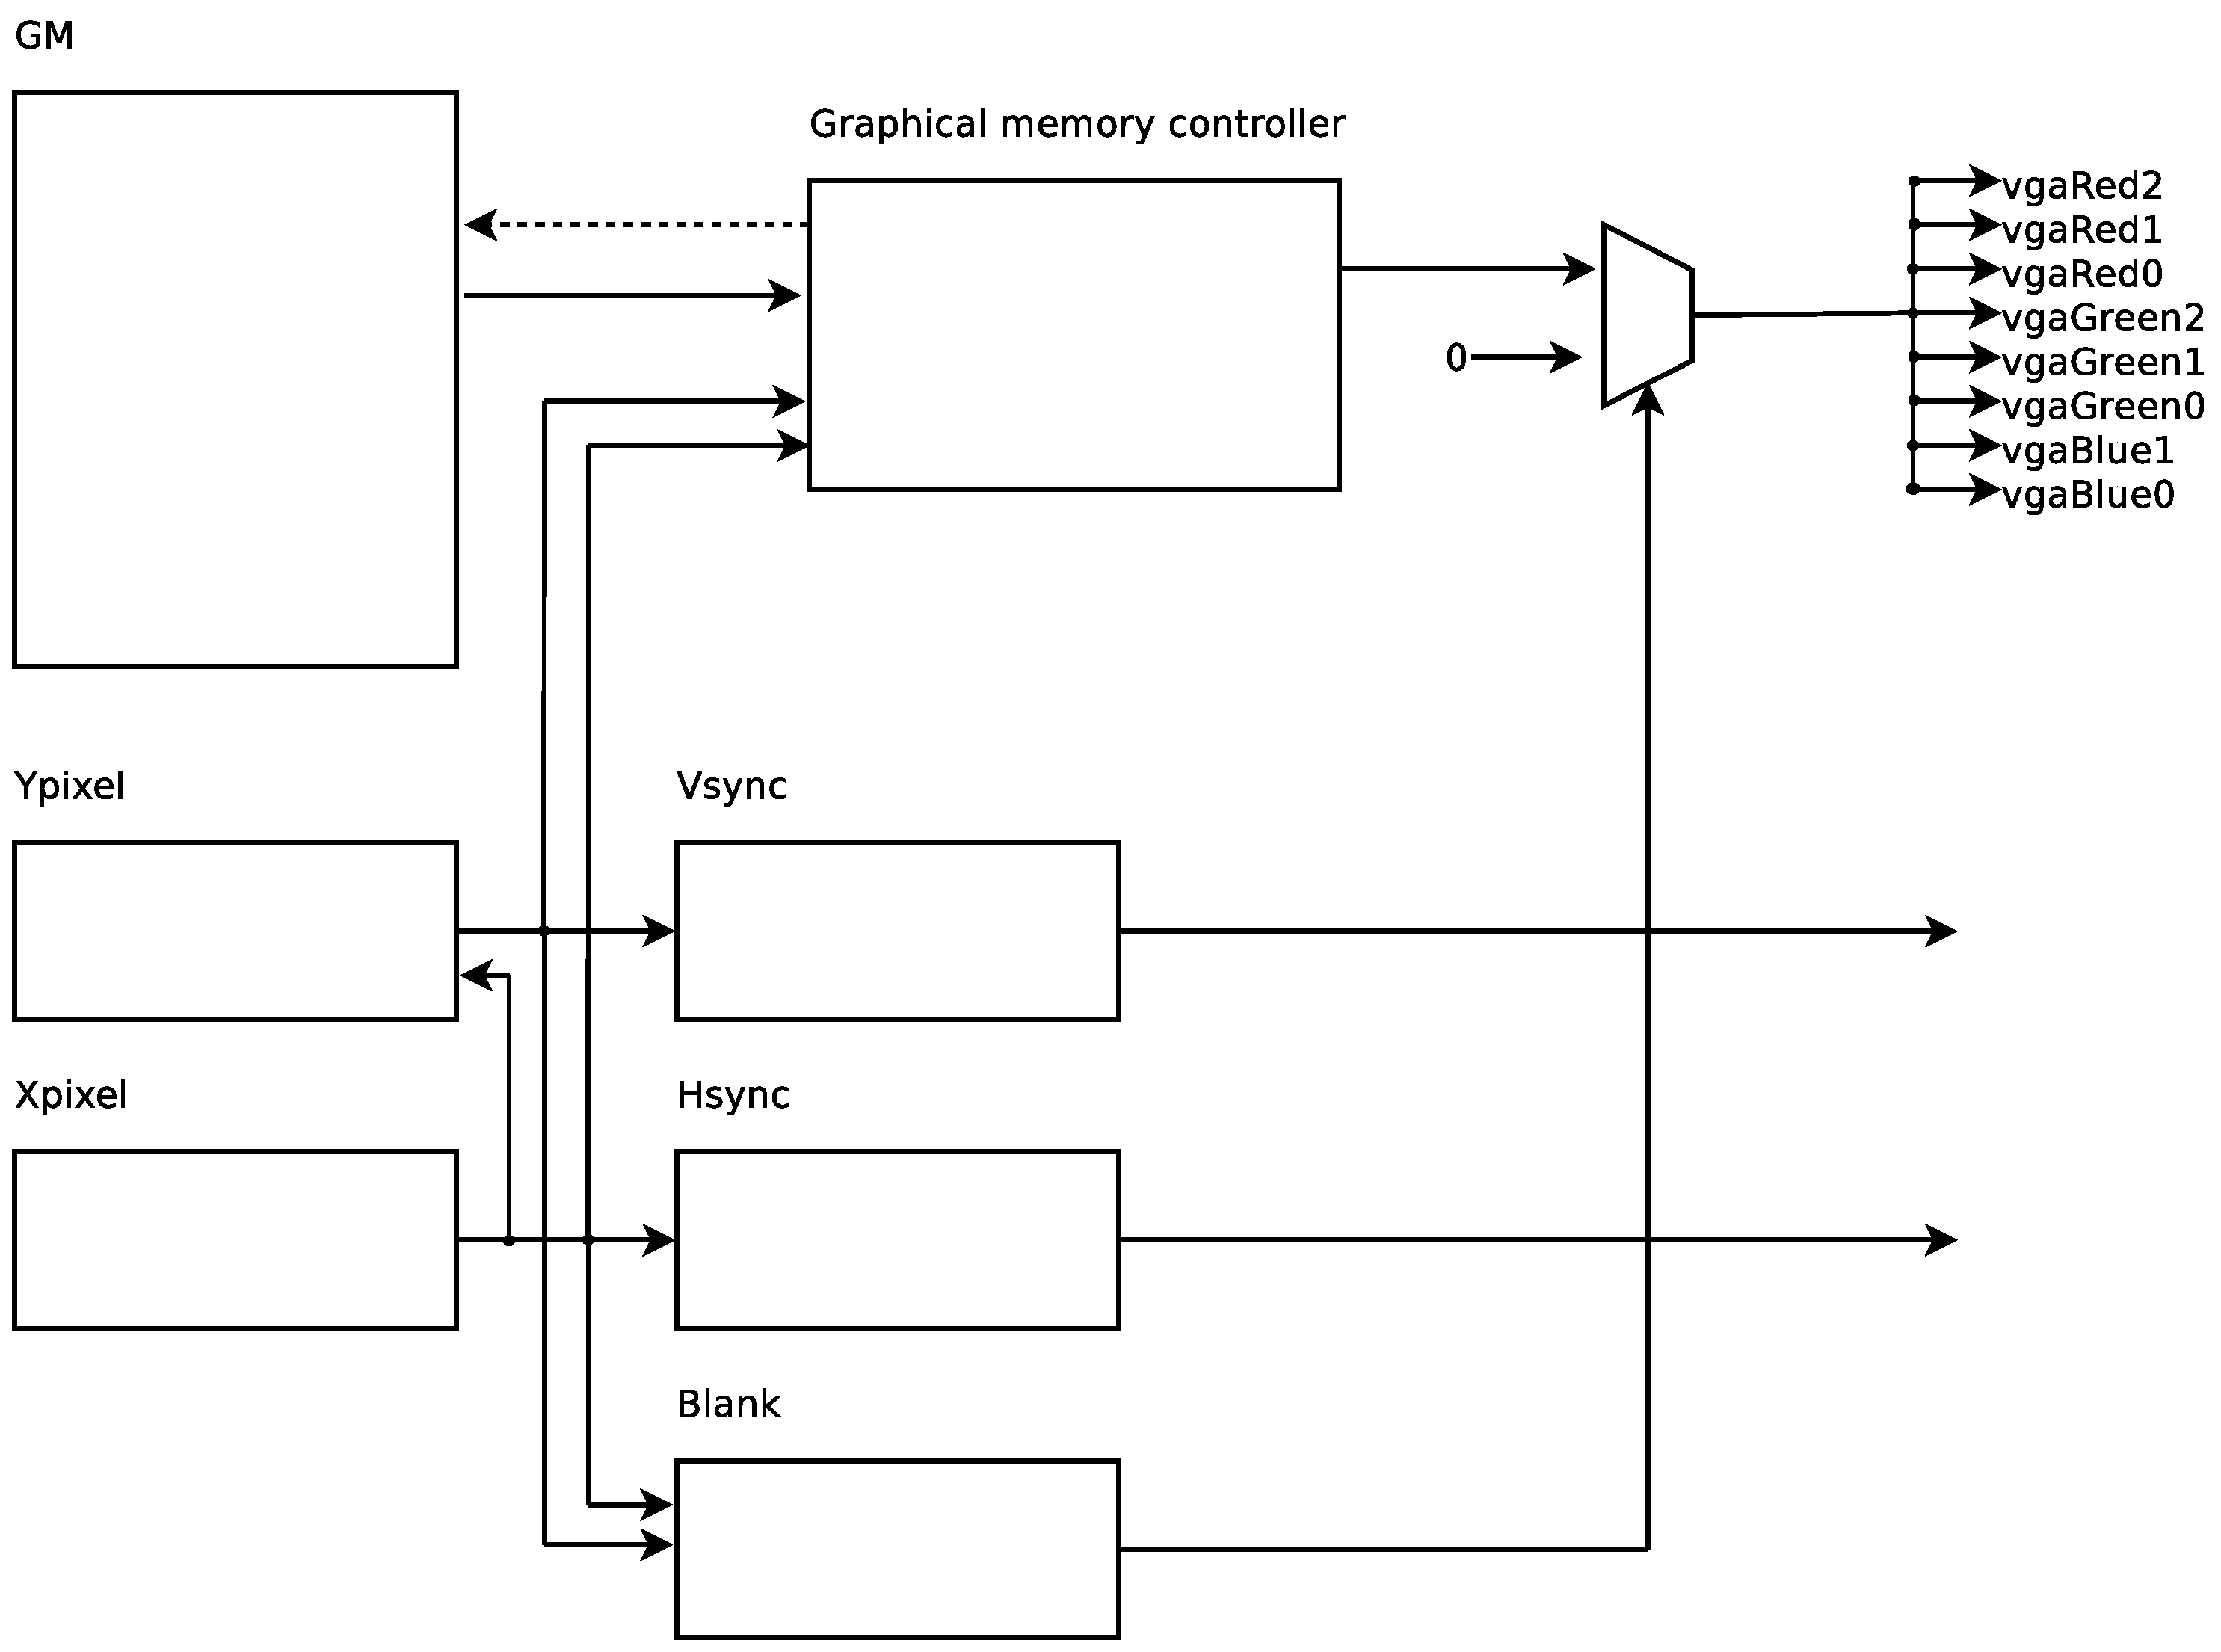
\includegraphics[scale=0.30]{../grafik/graphics.eps}
			\caption{VGA styrenhet}
			\label{fig:vga}
		\end{figure}
	\end{center}
Ovan ses ett översiktligt blockschema på VGA enheten. Enheten stödjer en upplösning på 640x480 pixlar och körs i 60Hz. Den stödjer två färger, svart och vit. Värderna som är valda medför att enheten måste ha en klocka på 25MHz. En spelpixel är definierad som 10x10 pixlar på VGA-skärmen, vilket resulterar i att den faktiska upplösningen är 64x48 pixlar. Grafikminnet är gjort så att en bit representerar en spelpixel. Det vill säga att fyra rader i minnet representerar en rad med spelpixlar på skärmen.
\subsection{I/O enheten}
	\begin{center}
		\begin{figure}[H]
    	\centering
			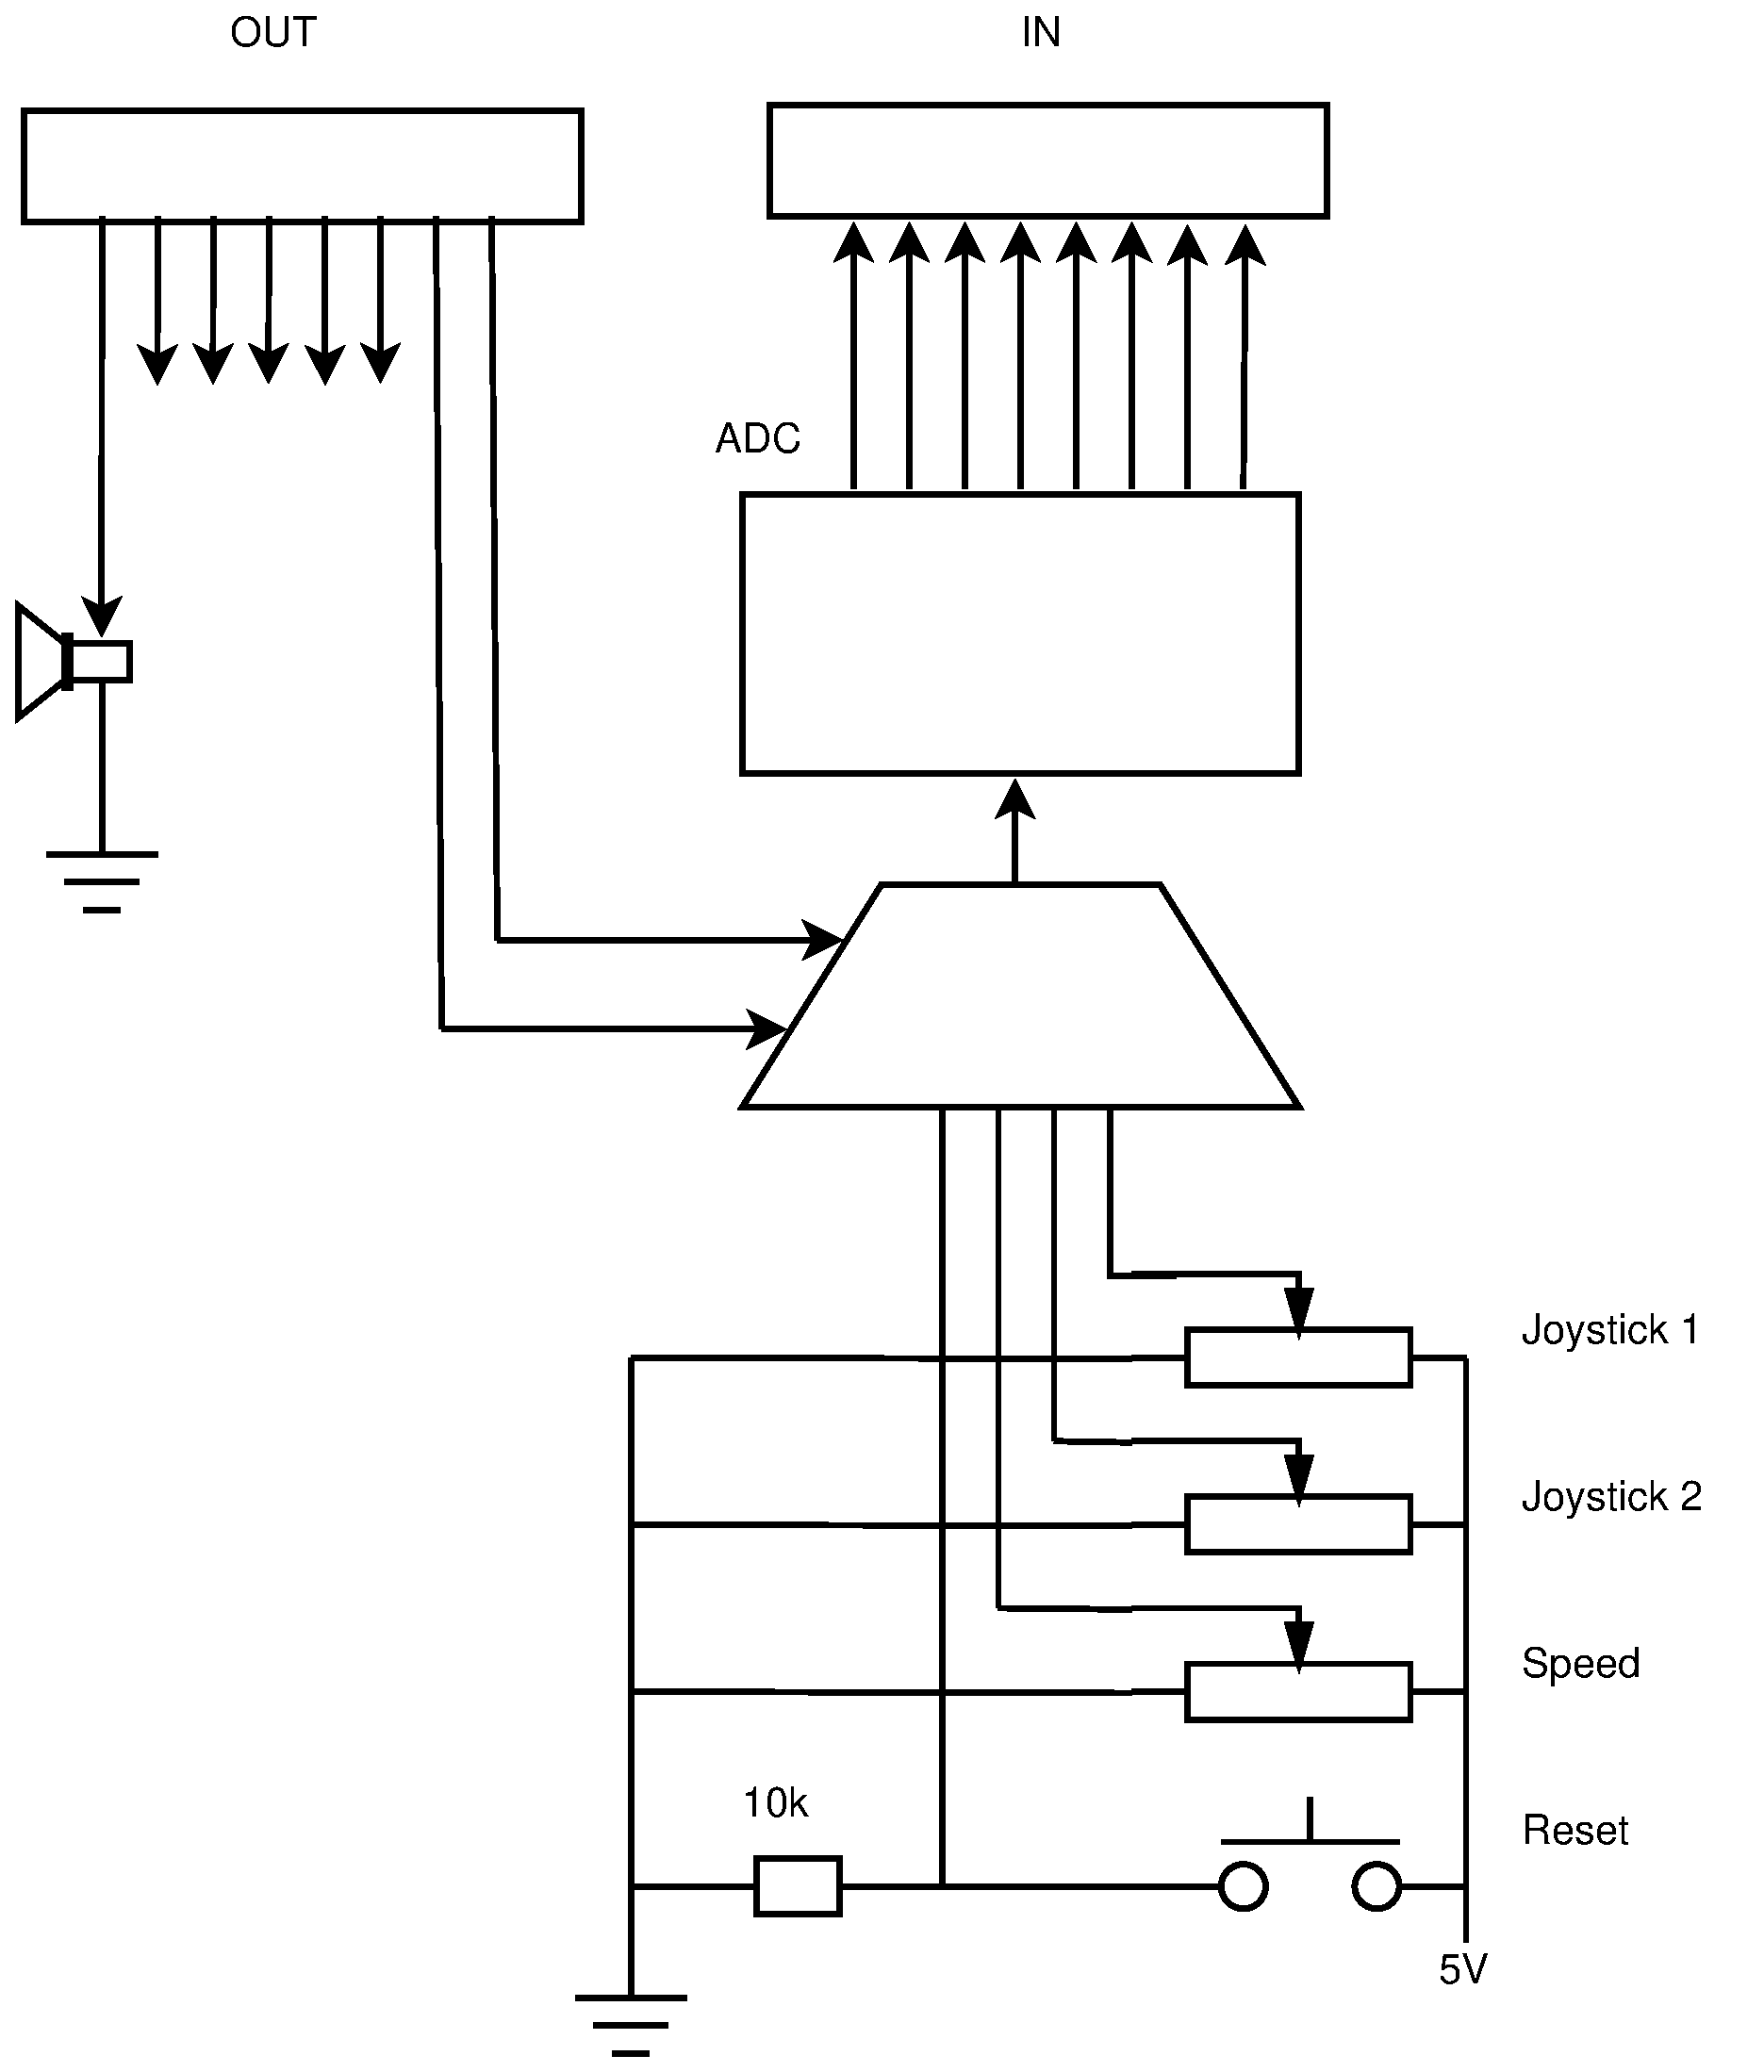
\includegraphics[scale=0.40]{../grafik/io.eps}
			\caption{IO design}
			\label{fig:joy}
		\end{figure}
	\end{center}
CPU:n har en 8 bitars ingång och en 8 bitars utgång som styrs av instruktionerna IN och OUT. Detta gör det möjligt att ha en extern AD-omvandlare och en analog mux för att kunna läsa av flera potentiometers. Dessa används för att styra staplarna i spelet.
Det är också möjligt att ha en extern reset knapp och hastighetskontroll. Dock är dessa funktioner inte implementerade.

